\section{Analysis}\label{sec:ana}
\vspace{\columnsep}

This section presents a review of the overall analysis process in the following 3 subsections:
an overview of the analysis can be found in section \ref{subsec:strategy}, the overall analysis processes including on/offline event selection and offline analysis routines can be found in section \ref{subsec:anaPrs}, and studies and updates specifically apply for this analysis can be found in section \ref{subsec:update}, respectively.

In general, most of the processes are the same as the previous \Xic $\rightarrow$ e\Xim analysis \cite{ana990_Xic0}, however, there are a few notable differences as well.

First of all, this analysis classifies the \pp 13 \TeV dataset into several categories by multiplicity. For this purpose, the events triggered by HMV0 are newly added and existing MB triggered events are sorted out by their multiplicity. There is a total of four categories (hereafter will be denoted as a "configuration") by the trigger and relevant V0M multiplicity percentile, as follows.

\begin{itemize}
    \small
    \item[] \blue{List of configurations by trigger and multiplicity} \vspace{1pt}
    \item[1.] MB + [0, 100]
    \item[2.] MB + [30, 100]
    \item[3.] MB + [0.1, 30]
    \item[4.] HMV0 + [0, 0.1]
\end{itemize}

Note that each configuration is treated independently: i.e., the processes for MB + [0, 100] and HMV0 + [0, 0.1] are separated in ROOT file level, from the offline event selection.

Second, since each configuration stands only for a part of the entire dataset, some global factors such as the V0 detector cross-section cannot be used (i.e., there's no guarantee that the V0 cross-section for MB inclusive is the same for MB + [0.1, 30]). This feature also causes similar problems for some analysis steps, such as feed-down correction.

Third and Finally, the final observable of this analysis is the baryon-to-meson ratio by using \Xic/\Dzero. Since this analysis relies on existing results \cite{ana993_D0} for its denominator (\Dzero), this feature restricts some analytical choices such as multiplicity percentile window of a configuration, INEL$>$0 condition, and \pt binning of spectra of interest.





\clearpage
%--------------------------------------------------------

\subsection{Analysis strategy} \label{subsec:strategy}
The chain of decay for \Xic $\rightarrow$ e\Xim is described in Eq. \ref{eq:s2_decay} and Fig. \ref{fig:s2_decay}.

\begin{equation}
    \Xi_{c}^{0}\xspace \rightarrow
    e^{+}\Xi^{-}\nu_{e} \rightarrow
    e^{+}(\pi^{-}\Lambda^{0})\nu_{e} \rightarrow
    e^{+}(\pi^{-}(p\pi^{-}))\nu_{e} 
    + c.c
    \label{eq:s2_decay}
\end{equation}
%
\begin{table}[h]
    \centering
    \small
    \begin{tabular}{c|c|c|c|c|c}
    \hline\hline
    %
    Particle & Quarks & Mass (\MeVmass) & Decay mode & BR (\%) & $c\tau$ \\\hline
    \Xic & dsc & 2470.91 $\pm$ 0.25 & \ensuremath{e^{+}\Xi^{-}\nu_{e}} & 1.8 $\pm$ 1.2 & 33.6 $\mu$m \\
    \X & dss & 1321.71 $\pm$ 0.07 & \ensuremath{\pi^{-}\Lambda^{0}} & 99.987 $\pm$ 0.035 & 4.91 cm \\
    \ensuremath{\Lambda^{0}} & uds & 1115.682 $\pm$ 0.006 & \ensuremath{p\pi^{-}} & 63.9 $\pm$ 0.5 & 7.89 cm \\
    %
    \hline\hline
    \end{tabular}
    \caption{Properties of particles of interest \cite{PDG}}
    \label{tab:particles}
\end{table}

\begin{figure}[h!]
    \centering
    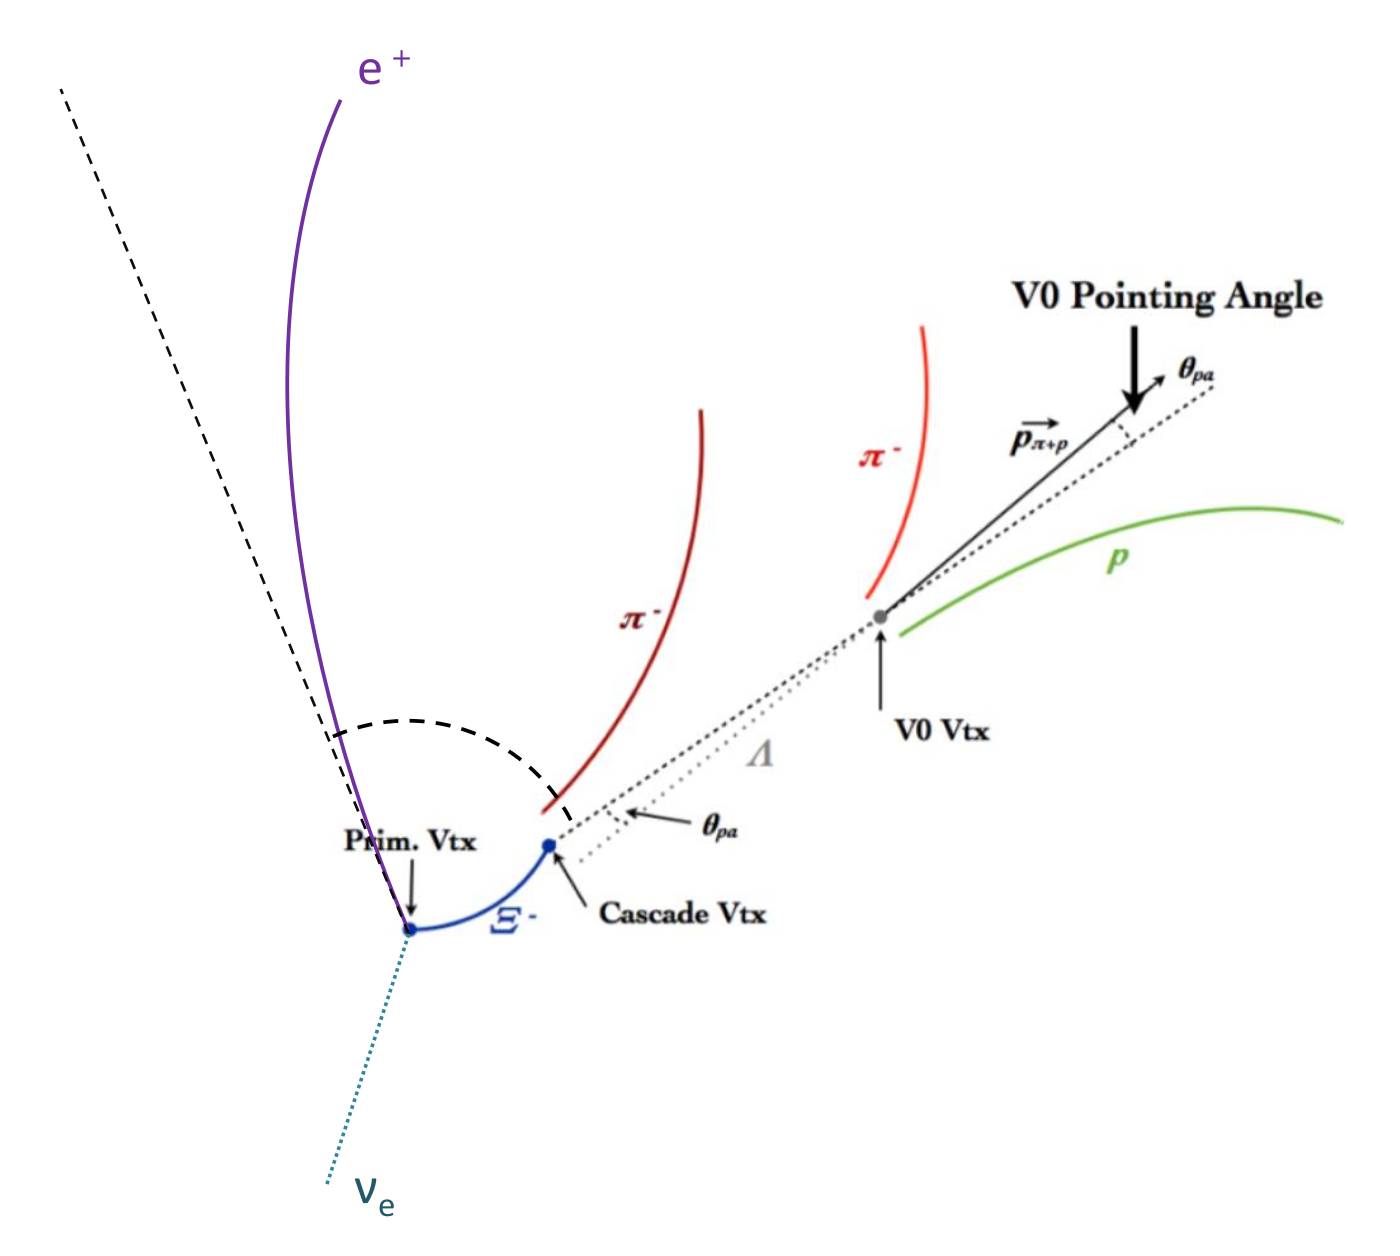
\includegraphics[width=0.50\textwidth]{plots/s2_strategy.png}
    \caption{Chain of \Xic $\rightarrow$ e\Xim decay}
    \label{fig:s2_decay}
\end{figure}

The strategy of measuring the \Xic can be summarized as follows.
%
\begin{itemize}
    \small
    \item[] \blue{Online event selection} \vspace{1pt}
    \item[-] Collect candidates of e-\Xim pair in loose conditions \vspace{\columnsep}
    \item[] \blue{Offline event selection} \vspace{1pt}
    \item[-] Apply eventwise cuts (e.g., sorting out by configuration)
    \item[-] Sort out candidates by quality (e.g., topology cut for \Xim) \vspace{\columnsep}
    \item[] \blue{Offline analysis} \vspace{1pt}
    \item[1.] Make e-\Xim pairs by charge sign: RS (right sign, sign is opposite to each other) or WS (wrong-sign), \\then obtain the signal distribution by RS - WS
    \item[2.] Correct efficiency for "prefilter" on electron candidates
    \item[3.] Correct the over-subtraction caused by \Xib
    \item[4.] Convert \pt of e-\Xim pair into \pt of \Xic by unfolding
    \item[5.] Correct efficiency for \Xic by using MC
    \item[6.] Correct for the prompt \Xic fraction
    \item[7.] Compute final observable
\end{itemize}
%
Further detailed information such as cut values can be found in the following section \ref{subsec:anaPrs}.





\clearpage
%--------------------------------------------------------

\subsection{Analysis process} \label{subsec:anaPrs}
\subsubsection{Online event selection} \label{subsubsec:onSel}
The conditions applied for the event selection via \textit{AliAnalysisTask} and ALICE \textit{Lego train} system are summarized in the following items. Note that the conditions are chosen very loosely, leaving fine filtering to the later offline event selection stage.

\begin{itemize}
    \small
    \item [] \blue{Eventwise cuts} \vspace{1pt}
    \item[-] 252000 $<$ run number
     \footnote{\textit{AliVEvent::GetRunNumber()}} $<$ 295000
     \item[-] Either MB or HMV0 trigger is fired
     \footnote{\textit{AliVEvent::kINT7, AliVEvent::kHighMultV0}}
     \item[-] Valid V0M multiplicity can be found
     \footnote{\textit{AliMultSelection::GetMultiplicityPercentile("V0M")}}
    \item[-] Primary vertex $|$z$|$ $<$ 10 (cm)
     \footnote{\textit{AliVVertex::GetZ()} $<$ 10.0}
    \item[-] Pileup rejection
     \footnote{\textit{AliRDHFCutsXictoeleXifromAODtracks::SetOptPileup(AliRDHFCuts::kRejectMVPileupEvent)}}
    %\item[-] Assign an \textit{AliNormalizationCounter} object for each configuration
\end{itemize}
%
\begin{itemize}
    \small
    \item[] \blue{Cuts for track (common)} \vspace{1pt}
    \item[-] AOD filter bit of 4 (standard cuts with very loose DCA)
    \footnote{\textit{AliAODTrack::TestFilterMask(AliAODTrack::kTrkGlobalNoDCA)}}
    % https://github.com/alisw/AliRoot/blob/master/STEER/AOD/AliAODTrack.h
    \item[-] \pt $>$ 0.5 (\GeVc) \footnote{\textit{AliAODTrack::Pt() $>$ 0.5)}}
    \item[-] $|\eta|$ $<$ 0.8 \footnote{\textit{AliAODTrack::Eta() $<$ 0.8}}
    \item[-] Number of TPC pID clusters $>$ 50
    \footnote{\textit{AliAODTrack::GetTPCsignalN() $>$ 50}}
    \item[-] Quality cuts
    \footnote{\textit{AliESDtrackCuts::SetClusterRequirementITS(AliESDtrackCuts::kSPD, AliESDtrackCuts::kBoth)}}
    \footnote{\textit{AliESDtrackCuts::SetDCAToVertex2D(true)}}
    \footnote{\textit{AliESDtrackCuts::SetMaxChi2PerClusterITS(36)}}
    \footnote{\textit{AliESDtrackCuts::SetMaxDCAToVertexXY(1.0)}}
    \footnote{\textit{AliESDtrackCuts::SetMaxDCAToVertexZ(2.0)}}
    \footnote{\textit{AliESDtrackCuts::SetMinNClustersITS(2)}}
    \footnote{\textit{AliESDtrackCuts::SetRequireTPCRefit(true)}}
    \footnote{\textit{AliESDtrackCuts::SetRequireITSRefit(true)}}
\end{itemize}
%
\begin{itemize}
    \small
    \item[] \blue{Cuts for cascade/V0 tracks} \vspace{1pt}
    \item[-] $|\sigma_{\rm TPC}| <$ 4
     \footnote{\textit{AliPIDResponse::NumberOfSigmasTPC() $<$ 4}}
    %\item[-] Reject charged $\Lambda$ %by mass tolerance of 0.008
    %\item[-] Valid decay lengths (both $\Xi$ and V0)
    \item[-] DCA of bachelor track to PV (primary vertex) $>$ 0.01 (cm)
     \footnote{\textit{AliAODcascade::DcaBachToPrimVertex()}}
    \item[-] DCA of V0 to PV $>$ 0.01 (cm)
     \footnote{\textit{AliAODcascade::DcaV0ToPrimVertex()}}
    \item[-] DCA of V0 daughters to PV $>$ 0.05 (cm)
     \footnote{\textit{AliAODcascade::Dca(Pos/Neg)ToPrimVertex()}}
    \item[-] (Both \Xim and V0) Daughters' DCA $<$ 1.68 (cm)
     \footnote{\textit{AliAODcascade::DcaXiDaughters(),
     AliAODcascade::DcaV0Daughters()}}
    \item[-] (Both \Xim and V0) Cosine of pointing angle $>$ 0.98
     \footnote{\textit{AliAODcascade::CosPointingAngle(),
     AliAODcascade::CosPointingAngleXi()}}
    \item[-] (Both \Xim and V0) Decay length $>$ 0.2 (cm)
     \footnote{Calculated from \textit{AliAODcascade::DecayVertex(Xi/V0)(X/Y/Z)}}
    \item[-] $\lambda$ mass tolerance: 0.008 (\GeVmass)
    \item[-] Reject \Omg baryon by mass
\end{itemize}
%
\clearpage
\begin{itemize}
    \small
    \item[] \blue{Cuts for electron track} \vspace{1pt}
    \item[-] Minimum \footnote{Minimum = {-4.3 + (1.17*\pt) - (0.094*\ensuremath{p_{\rm T^{2}}})},
    fix multiplied \pt to 5.0 if \pt $>$ 5.0} $< |\sigma_{\rm TPC}| <$ 3
    \item[-] $|\sigma_{\rm TOF}| <$ 3
     \footnote{\textit{AliPIDResponse::NumberOfSigmasTOF() $<$ 3}}
    \item[-] m$_{\,e^{+}e{-}}$ $<$ 0.05 (\GeVmass)
\end{itemize}
%

The total number of events processed during the online selection is summarized in table \ref{tab:nEvents}.
Note that the number of events was independently counted for each configuration by assigning an \textit{AliNormalizationCounter} object to each configuration. Also, the vertex finding efficiency was applied \footnote{\textit{AliNormalizarionCounter::GetNEventsForNorm()}} for the values.

\vspace{\columnsep}
\begin{table}[h]
    \centering
    \small
    \begin{tabular}{l|c|c|c}
    \hline\hline
    \multirow{2}{*}{Configuration} & \# of events ($B$) & \# of events ($B$) & Difference \\
    & (default) & (INEL$>$0) & ($|$default - INEL$>$0$|$ / default) \\\hline
    MB + [0, 100]   & 1.794 & 1.691 & 0.0574 \\\hline
    MB + [30, 100]  & 1.287 & 1.188 & 0.0769 \\\hline
    MB + [0.1, 30]  & 0.502 & 0.501 & 0.0020 \\\hline
    HMV0 + [0, 0.1] & 0.499 & 0.499 & 0.0000 \\
    \hline\hline
    \end{tabular}
    \caption{Total number of events processed for each configuration}
    \label{tab:nEvents}
\end{table}





\vspace{\columnsep}
%\clearpage
%--------------------------------------------------------
\subsubsection{Offline event selection} \label{subsubsec:offSel}
A ROOT file with Tree based structure is generated as a result of previous online event selection. The conditions applied to collect the e-\Xim pair candidates are summarized in the following item and tables \ref{tab:ePID} - \ref{tab:eXiPair}.
All selection conditions except the eventwise cuts are categorized in five levels by its tightness: vloose (very loose), loose, stand (standard), tight, and vtight, respectively. As the name indicates, stand is the default condition of the analysis.
Note that the offline selection performed independently by sample type and configuration (e.g., MB + [0, 100] for data). The weighting on generated \pt (section \ref{subsubsec:weighting}) also performed at this stage.

\begin{itemize}
    \small
    \item [] \blue{Eventwise cuts (for each configuration)} \vspace{1pt}
    \item[-] Target trigger is fired (e.g., MB)
    \item[-] V0M multiplicity is within the range (e.g., 0.1 $<$ multiplicity percentile $<$ 30)
    \item[-] INEL$>$0
    \item[-] electron mass $>$ 0.05 (\GeVmass)
    \item[-] $\Xi$ mass tolerance: $\pm$ 0.008 (\GeVmass)
    %\item[-] $\Xi$ mass within tolerance: 1.32171 $\pm$ 0.008 (\GeVmass)
    \item[-] e-$\Xi$ pair mass $>$ 1.3 (\GeVmass)
    \footnote{\textit{AliPPVsMultUtils::IsINELgtZERO(AliVEvent)}}
    %\footnote{MC: \textit{AliAODMCParticle::IsPhysicalPrimary() \&\& Charge() != 0 \&\& $|\eta|$ $<$ 1.0}}
\end{itemize}

\vspace{\columnsep}
\begin{table}[hb]
    \centering
    \small
    \begin{tabular}{r|c|c|c}
    \hline\hline
    %ut (level\textbackslash item) & $\sigma_{\rm TPC}$ min ($\geq$) & $\sigma_{\rm TPC}$ max ($\leq$) & $|\sigma_{\rm TOF}|$ ($\leq$) \\\hline
    \multirow{2}{*}{Cut (level\textbackslash item)} & $\sigma_{\rm TPC}$ min ($\geq$) & 
    \multirow{2}{*}{$\sigma_{\rm TPC}$ max ($\leq$)} & 
    \multirow{2}{*}{$|\sigma_{\rm TOF}|$ ($\leq$)} \\
    & * Variable \pt is fixed to 5.0 if \pt $>$ 5.0 & & \\\hline
    vloose & {-4.3 + (1.17*\pt) - (0.094*\ensuremath{p_{\rm T^{2}}})} & \multirow{5}{*}{3} & \multirow{5}{*}{3} \\\cline{1-2}
    loose  & {-4.1 + (1.17*\pt) - (0.094*\ensuremath{p_{\rm T^{2}}})} & & \\\cline{1-2}
    stand  & {-3.9 + (1.17*\pt) - (0.094*\ensuremath{p_{\rm T^{2}}})} & & \\\cline{1-2}
    tight  & {-3.7 + (1.17*\pt) - (0.094*\ensuremath{p_{\rm T^{2}}})} & & \\\cline{1-2}
    vtight & {-3.5 + (1.17*\pt) - (0.090*\ensuremath{p_{\rm T^{2}}})} & & \\
    \hline\hline
    \end{tabular}
    \caption{Table of cuts for electron pID in offline selection%. The variable \pt being multiplied in the column $\sigma_{\rm TPC}$ min is fixed to 5.0 if the \pt $>$ 5.0
    }
    \label{tab:ePID}
\end{table}
%
\begin{table}[ht]
    \centering
    \small
    \begin{tabular}{l|c|c|c|c|c}
    \hline\hline
    Cut (item\textbackslash level) & vloose & loose & stand & tight & vtight \\\hline
    \# of crossed rows ($>$)                        & 65 & 65 & 70 & 75 & 85 \\\hline
    \# of TPC pID clusters ($>$)                    & 40 & 45 & 50 & 55 & 60 \\\hline
    \# of crossed rows/\# of TPC pID clusters ($>$) & 0.70 & 0.75 & 0.80 & 0.85 & 0.90 \\\hline 
    \# of ITS clusters ($\geq$)                     & \multicolumn{5}{c}{3} \\
    \hline\hline
    \end{tabular}
    \caption{Table of cuts for electron reconstruction in offline selection}
    \label{tab:eReco}
\end{table}
%
\begin{table}
    \centering
    \small
    \begin{tabular}{l|c|c|c|c|c}
    \hline\hline
    Cut (item\textbackslash level) & vloose & loose & stand & tight & vtight \\\hline
    Decay length of \Xim (cm) ($>$)         & 0.5 & 0.5 & 0.5 & 0.6 & 0.7 \\\hline
    Decay length of V0 (cm) ($>$)           & 1.10 & 1.55 & 2.67 & 3.60 & 4.39 \\\hline
    DCA of bachelor track to PV (cm) ($>$)  & 0.05 & 0.05 & 0.07 & 0.09 & 0.11 \\\hline
    DCA of V0 to PV (cm) ($>$)              & 0.05 & 0.07 & 0.09 & 0.10 & 0.12 \\\hline
    DCA of V0 daughters to PV (cm) ($>$)    & 0.05 & 0.07 & 0.095 & 0.11 & 0.13 \\\hline
    Cosine of pointing angle (both \Xim and V0) ($>$) & 0.98 & 0.981 & 0.983 & 0.9839 & 0.985 \\
    \hline\hline
    \end{tabular}
    \caption{Table of cuts for \Xim pID by topology in offline selection}
    \label{tab:XiPID}
\end{table}
%
\begin{table}
    \centering
    \small
    \begin{tabular}{l|c|c|c|c|c}
    \hline\hline
    Cut (item\textbackslash level) & vloose & loose & stand & tight & vtight \\\hline
    \# of crossed rows (V0 proton) ($>$) & \multirow{3}{*}{66} & \multirow{3}{*}{66} &
    \multirow{3}{*}{70} & \multirow{3}{*}{70} & \multirow{3}{*}{74} \\
    \# of crossed rows (V0 \ensuremath{\pi}\xspace) ($>$) & & & & & \\
    \# of crossed rows (cascade \ensuremath{\pi}\xspace) ($>$) & & & & & \\\hline
    \# of crossed rows/findable (V0 proton) ($>$) & \multirow{3}{*}{0.74} & \multirow{3}{*}{0.77} & \multirow{3}{*}{0.77} & \multirow{3}{*}{0.79} & \multirow{3}{*}{0.79} \\
    \# of crossed rows/findable (V0 \ensuremath{\pi}\xspace) ($>$) & & & & & \\
    \# of crossed rows/findable (cascade \ensuremath{\pi}\xspace) ($>$) & & & & & \\
    \hline\hline
    \end{tabular}
    \caption{Table of cuts for \Xim reconstruction in offline selection}
    \label{tab:XiReco}
\end{table}
%
\begin{table}[hb]
    \centering
    \small
    \begin{tabular}{l|c|c|c|c|c}
    \hline\hline
    Cut (item\textbackslash level) & vloose & loose & stand & tight & vtight \\\hline
    Mass (\GeVmass) ($<$) & N/A & 2.7 & 2.5 & 2.3 & N/A \\\hline
    Opening angle (\degree) ($>$) & N/A & N/A & 90 & 70 & N/A \\
    \hline\hline
    \end{tabular}
    \caption{Table of cuts for e-\Xim pair in offline selection}
    \label{tab:eXiPair}
\end{table}





\clearpage
%--------------------------------------------------------
\subsubsection{Offline analysis} \label{subsubsec:offAna}
This section shows a series of analysis routines to reach the desired observable. Although the final physics observable of the analysis is the baryon-to-meson ratio by \Xic/\Dzero, the desired observable of this section is the corrected invariant cross-section of the \Xic, as we rely on existing result for \Dzero.

Note that only the plots for configuration MB + [0, 100] will be presented as an example: check appendix \ref{sec:appB} for other configurations.

\vspace{\columnsep}
\paragraph{\blue{Signal extraction by RS-WS}}\mbox{}\\[1pt]
The mass of \Xic is 2470.91 $\pm$ 0.25 (\MeVmass) \cite{PDG}, however, due to the presence of neutrino in this decay mode (\Xic $\rightarrow$ e$\Xi \nu_{e}$) one cannot expect to observe a distinct mass peak, 
thus the conventional signal yields extraction by using the peak cannot be used. As an alternative, we depend on the sign of e\Xim pair, by subtracting the WS (Wrong Sign, charge sign of e = \Xim) distribution from the RS (Right Sign, e $\neq$ \Xim).

Fig. \ref{fig:s2_RSWS} shows the distribution of RS/WS pairs by \pt bin and the resulting signal distribution by RS-WS. As the distributions show, the statistics are in general poor for \pt $>$ 8, and very scarce for \pt $>$ 12.

\vspace{\columnsep}
\begin{figure}[h!]
    \centering
    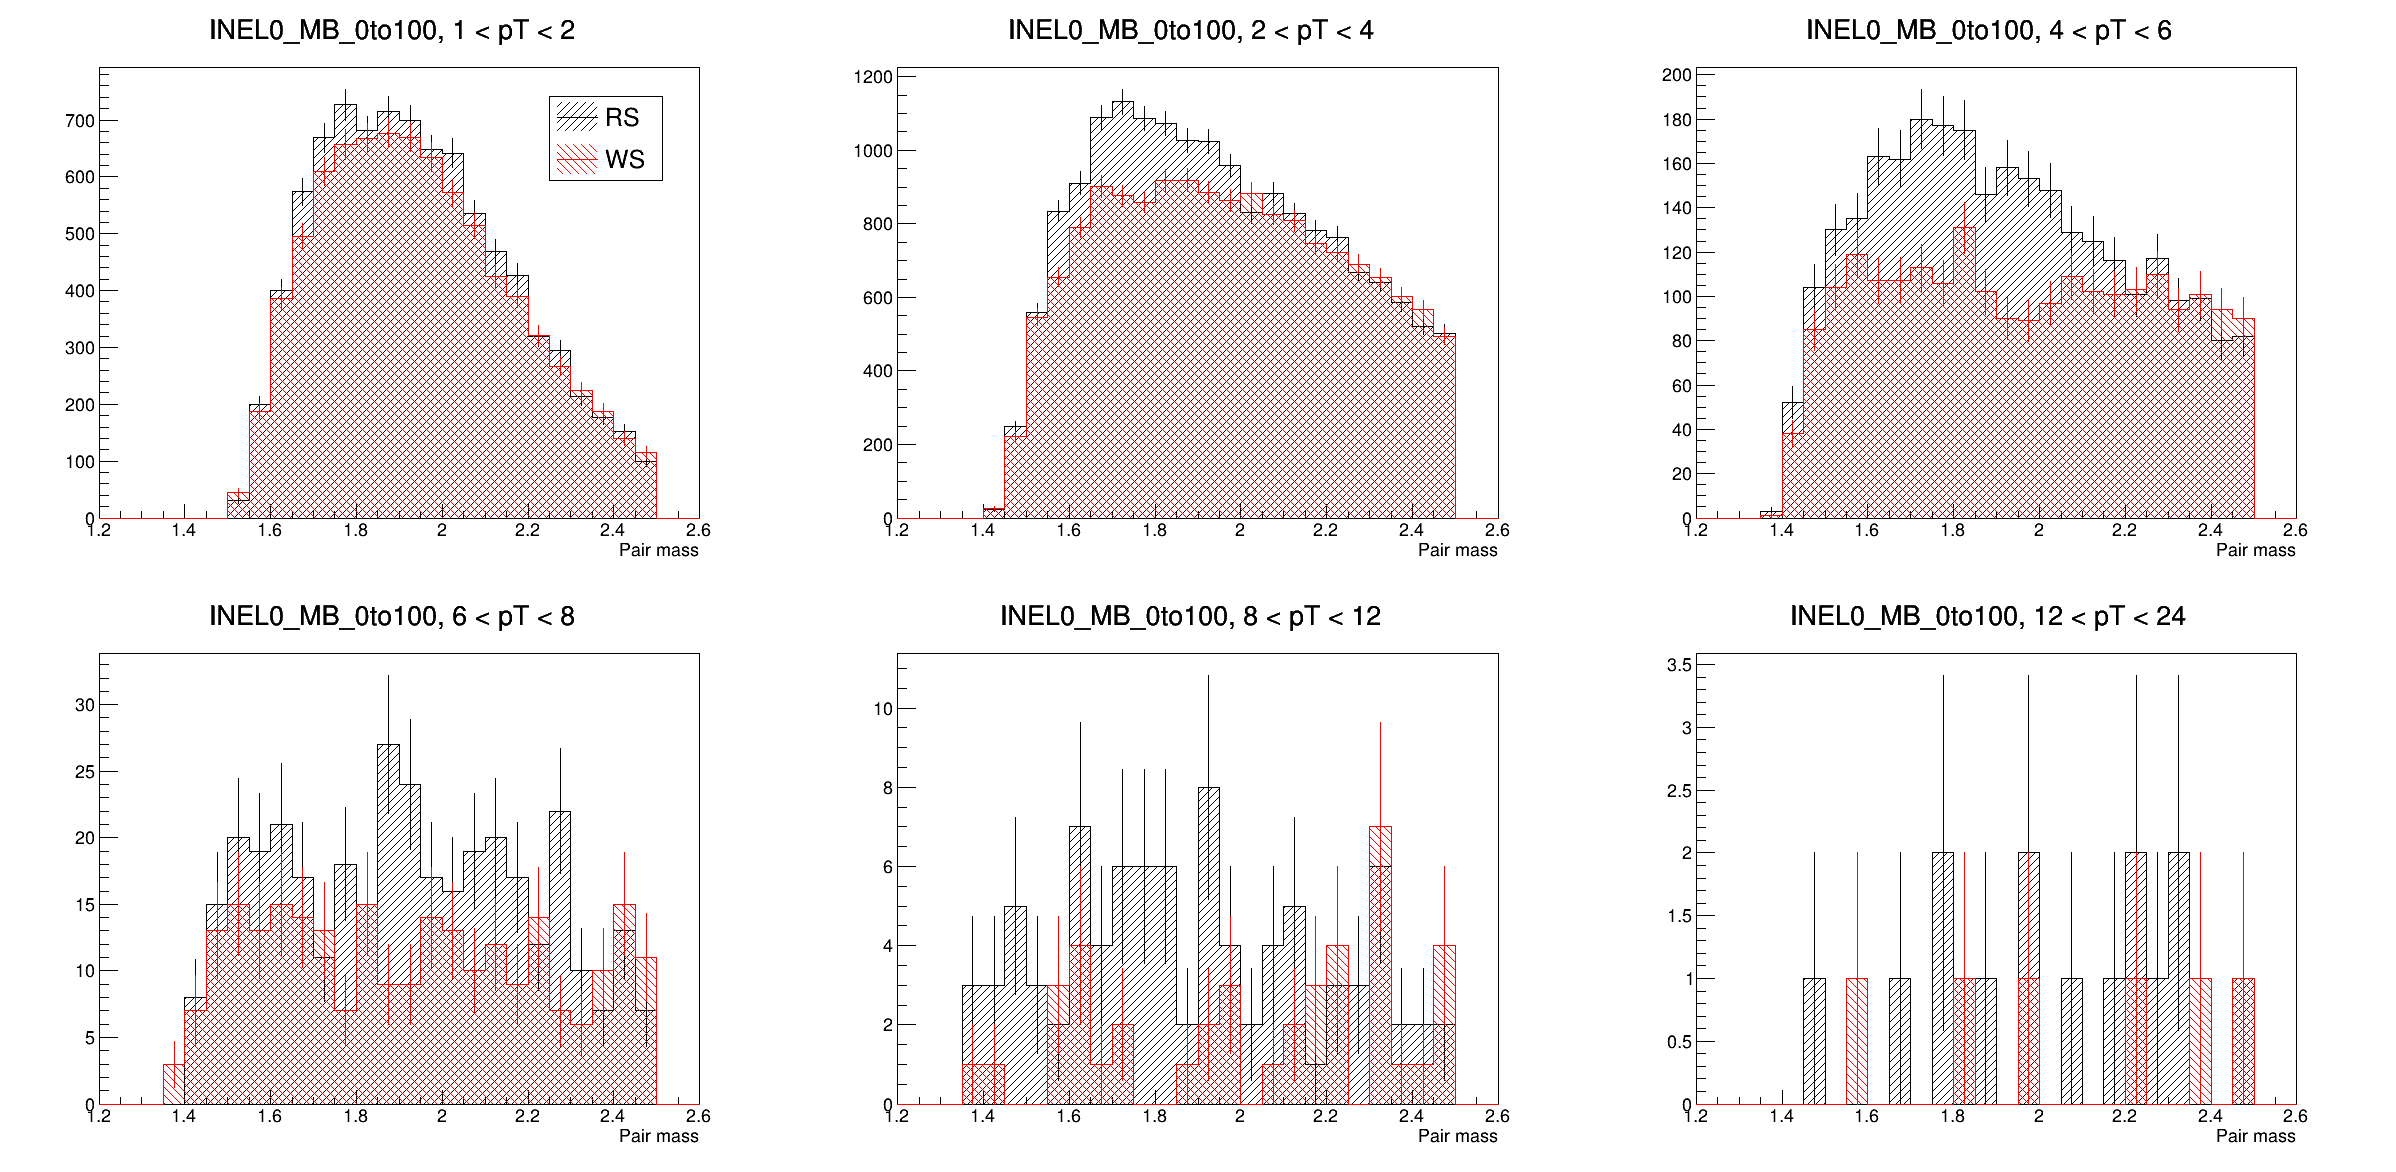
\includegraphics[width=0.90\textwidth]{plots/s2_RSmWS_INEL0_MB_0to100.png} \\\vspace{2pt}
    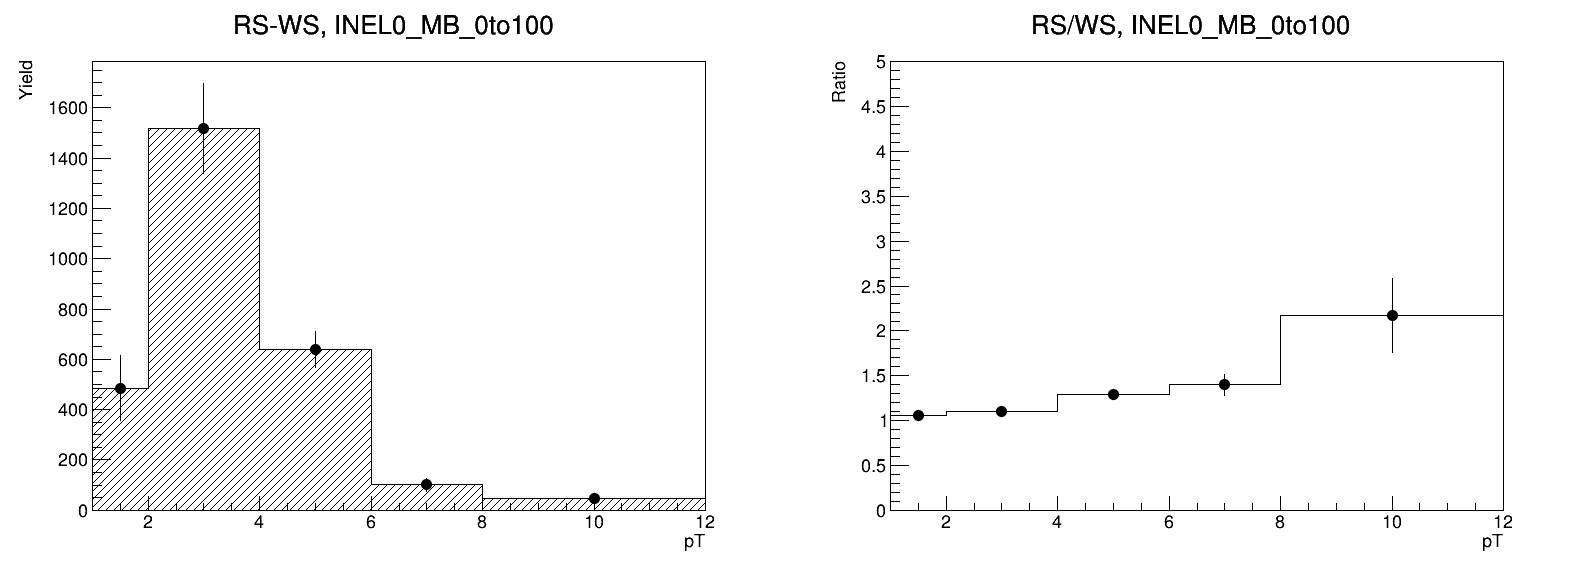
\includegraphics[width=0.95\textwidth]{plots/s2_RSdWS_INEL0_MB_0to100.png}
    \caption{\pt distributions of e\Xim pairs by sign (RS or WS) (top 6), extracted signal by RS-WS (bottom left), and ratio of RS/WS (bottom right). Only the configuration MB + [0, 100] is shown.}
    \label{fig:s2_RSWS}
\end{figure}

\clearpage
%++++++++++++++++++++++++++++++++++++++++++++

\vspace{\columnsep}
\paragraph{\blue{Prefilter efficiency correction}}\mbox{}\\[1pt]
A portion of signal electrons can be accidentally rejected by the applied electron track selection cuts (prefilter) during the online event selection. The definition of prefilter efficiency for the correction is as follows.

\begin{equation}
    \epsilon_{\,\text{\rm prefilter}} =
    \frac{N_{e\Xim} \text{\rm \,(prefilter on, same-sign pairs)}}{N_{e\Xim} \text{\rm \,(prefilter off})}
\end{equation}

The numerator indicates the number of e\Xim pairs collected with prefilter applied while the denominator is not. Also, for the numerator, the backgrounds yields (e-\Xim pairs with the same sign) were utilized to prevent large fluctuation from the poor statistics of signals (e-\Xim pairs with different signs).

Fig. \ref{fig:s2_preFEff} shows the estimated prefilter efficiency and the signal yields before and after the correction.

\vspace{\columnsep}
\begin{figure}[h]
    \centering
    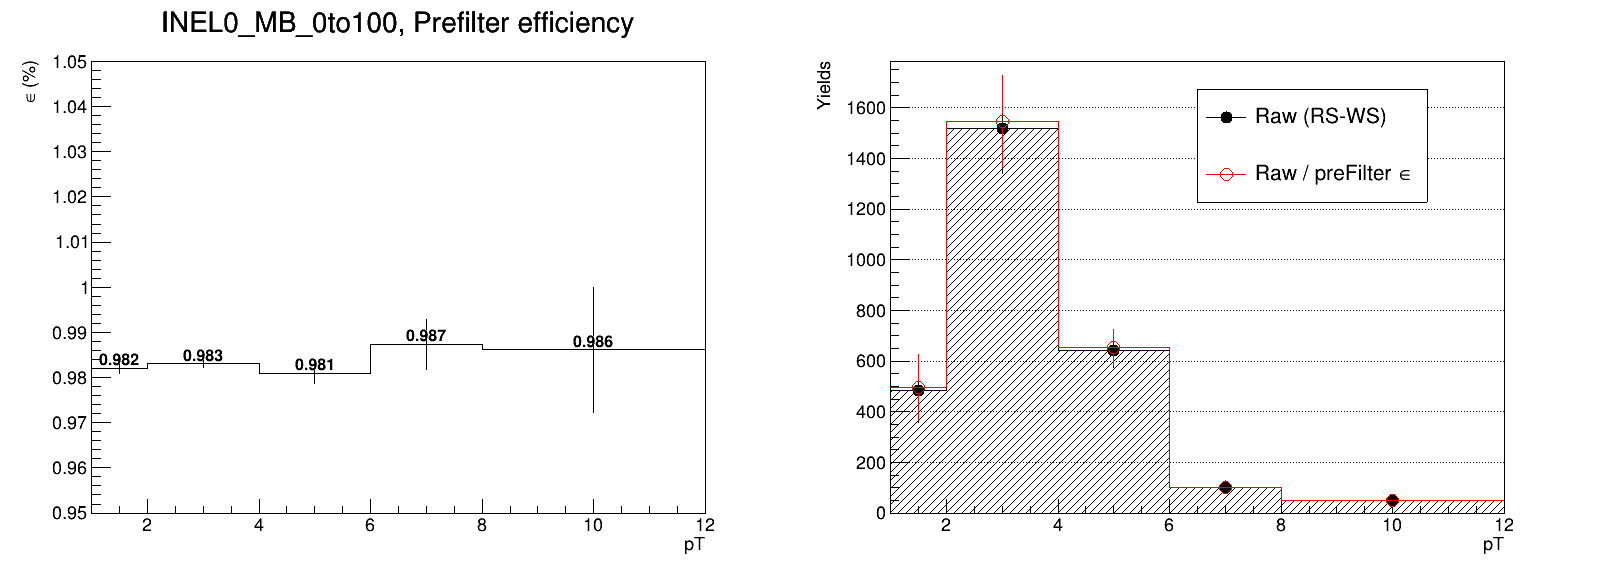
\includegraphics[width=0.95\textwidth]{plots/s2_preFCorr_INEL0_MB_0to100.png}
    \caption{Prefilter efficiency (left) and (RS-WS) yields before and after the correction (right)}
    \label{fig:s2_preFEff}
\end{figure}

%++++++++++++++++++++++++++++++++++++++++++++

\clearpage
\paragraph{\blue{\Xib over-subtraction correction}}\mbox{}\\[1pt]
\red{TBU}

\iffalse
- Uses 7 TeV CMS Lb \\
- Scale it up (7 $\rightarrow$ 13 TeV) by using FONLL\_B \\
- Normalize by using \# of events (normalization factor) and "V0 detector cross-section" \\
  (* V0 xSec is estimated for inclusive MB: would the xSec valid for HMV0 or specific mult. percentile?) \\
- Estimate efficiency of Xib (Xib generated vs. Xib reco) by using MC \\
  (* problem 1: Xib\_gen is prepared in train level) \\
  (* problem 2: Xib\_reco affected by the applied MC scaling factor (MB+[0, 100] != HMV0+[0,0.1]))
- Syst. err: cut tightness (std vs. vtight : applies to the Xib\ reco) \\
\fi
%
\begin{figure}[h]
    \centering
    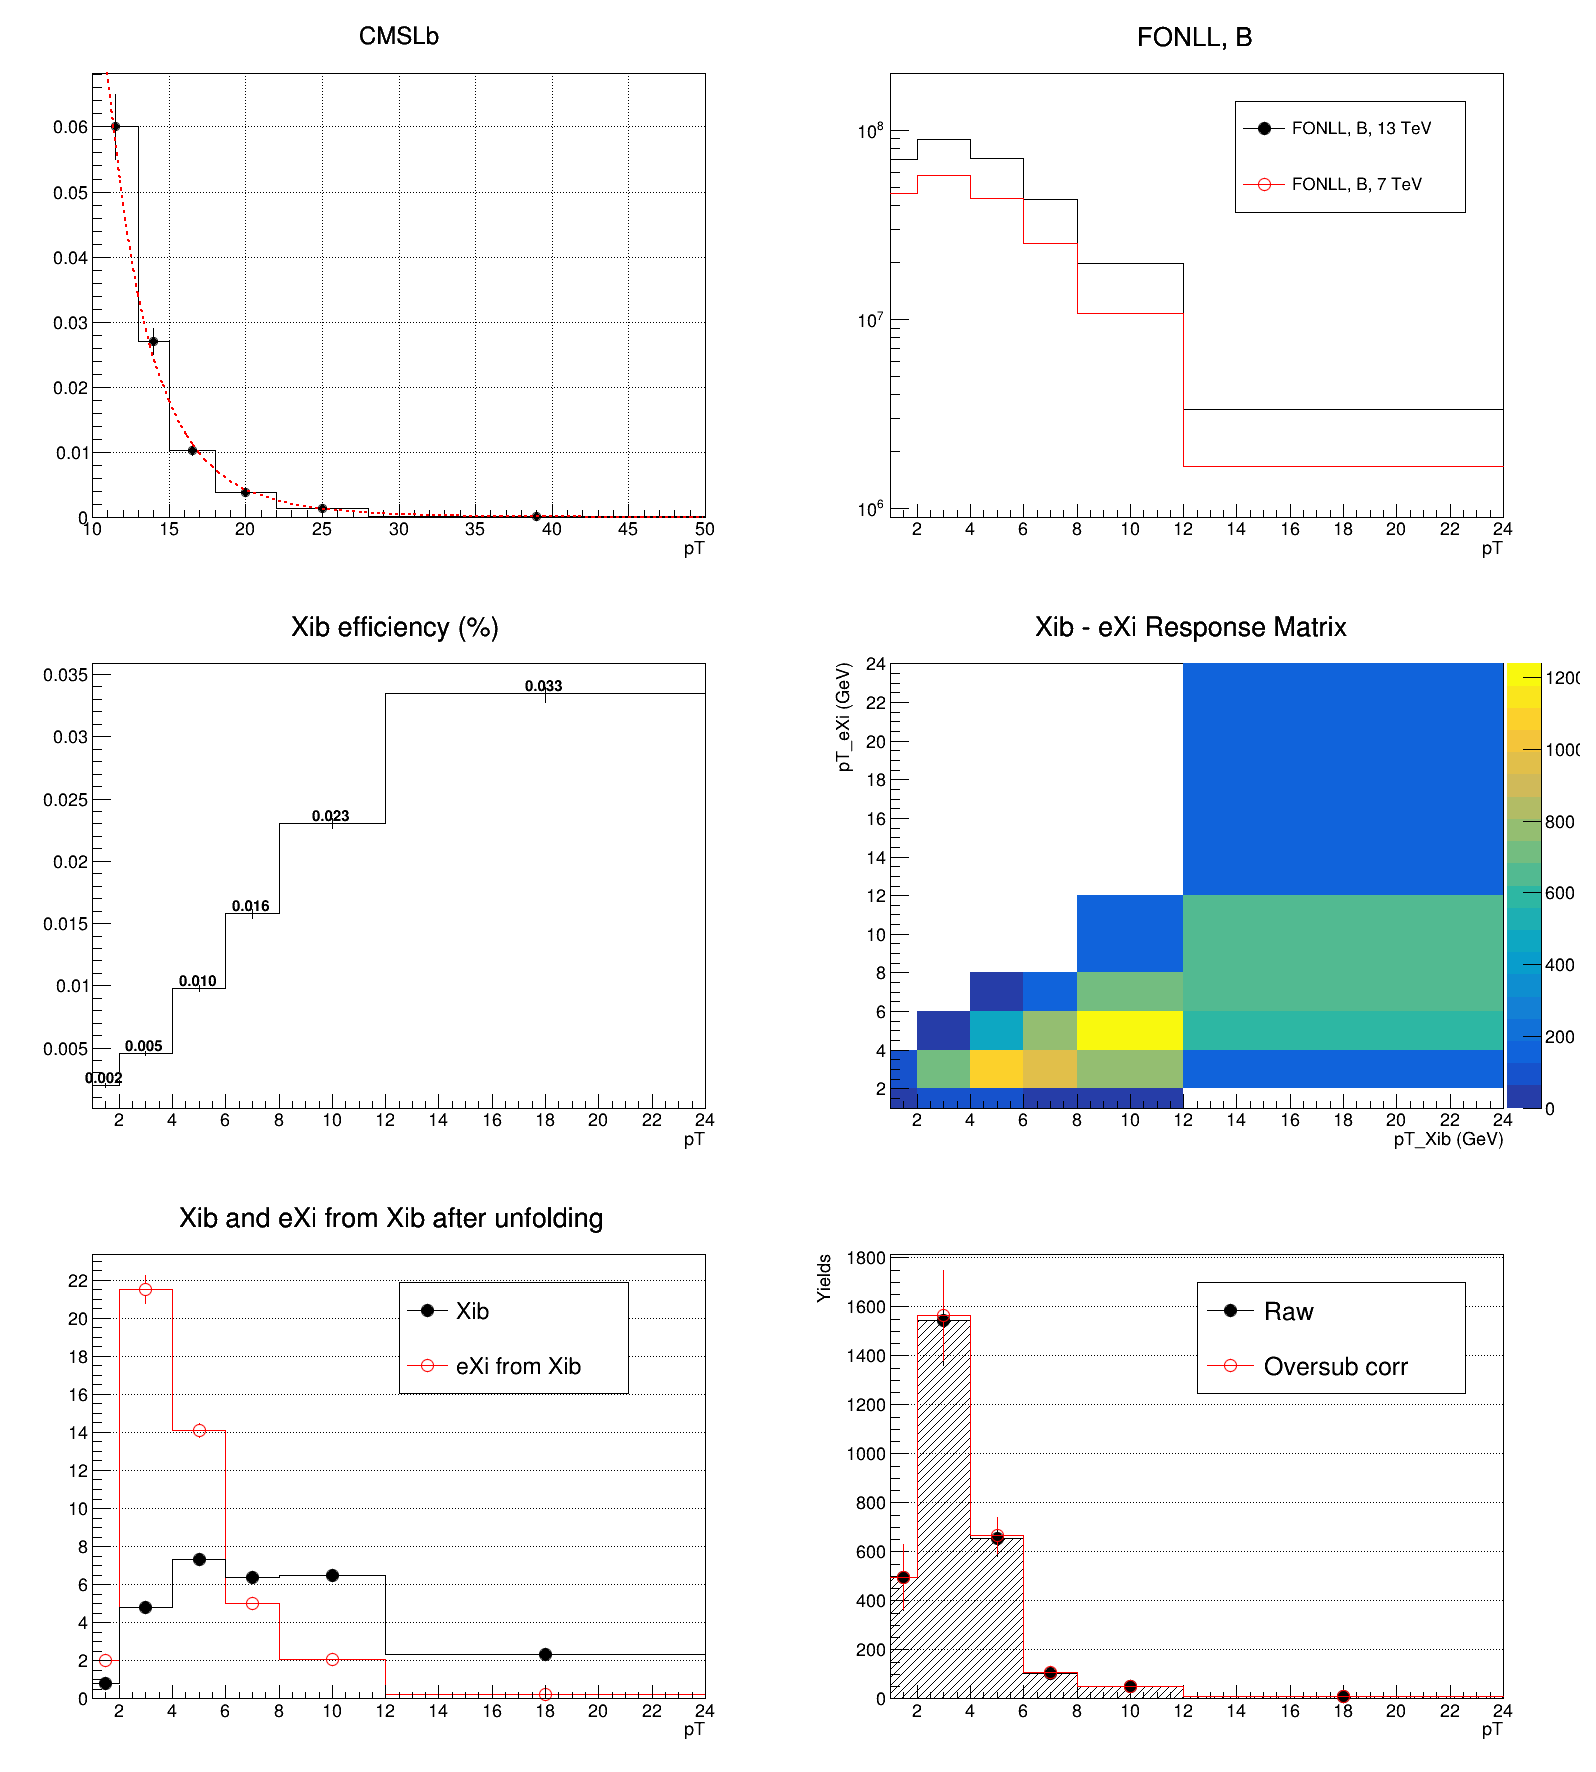
\includegraphics[width=0.95\textwidth]{plots/s2_c1b_Bayes_stand3_INEL0_MB_0to100_bCorr.png}
    \caption{\red{TBU}}
    \label{fig:s2_bCorr}
\end{figure}

\clearpage
%++++++++++++++++++++++++++++++++++++++++++++

\vspace{\columnsep}
\paragraph{\blue{Unfolding}}\mbox{}\\[1pt]
The unfolding can be explained as 'rewinding the distortion on the signal' by using truth information based on MC. By using the well-defined MC sample (PYTHIA8) and the same reconstruction process between the data and MC, the following relationship can be established between the measured quantity \textit{M} and the true quantity \textit{T}.

\vspace{\columnsep}
\centerline{\textit{M} = \textit{R} * \textit{T}}

The quantity \textit{R} is the Response Matrix of the detector which reflects the discrepancy between \textit{M} and \text{T} for given conditions (e.g., detector acceptance, etc). Note that the default method of the unfolding is Bayesian combined with an iterative procedure.

The subject variable of the unfolding is the \pt of the \Xic. Since the decay mode (\Xic $\rightarrow$ $e\Xi\nu_{e}$) includes a neutrino which cannot be measured with ALICE detectors, the unfolding is inevitably required to convert the measured e-\Xim pair's \pt to the one of \Xic.

Fig. \ref{fig:s2_unfolding} shows the applied Response Matrix and the yields before and after the unfolding.

\vspace{\columnsep}
\begin{figure}[h]
    \centering
    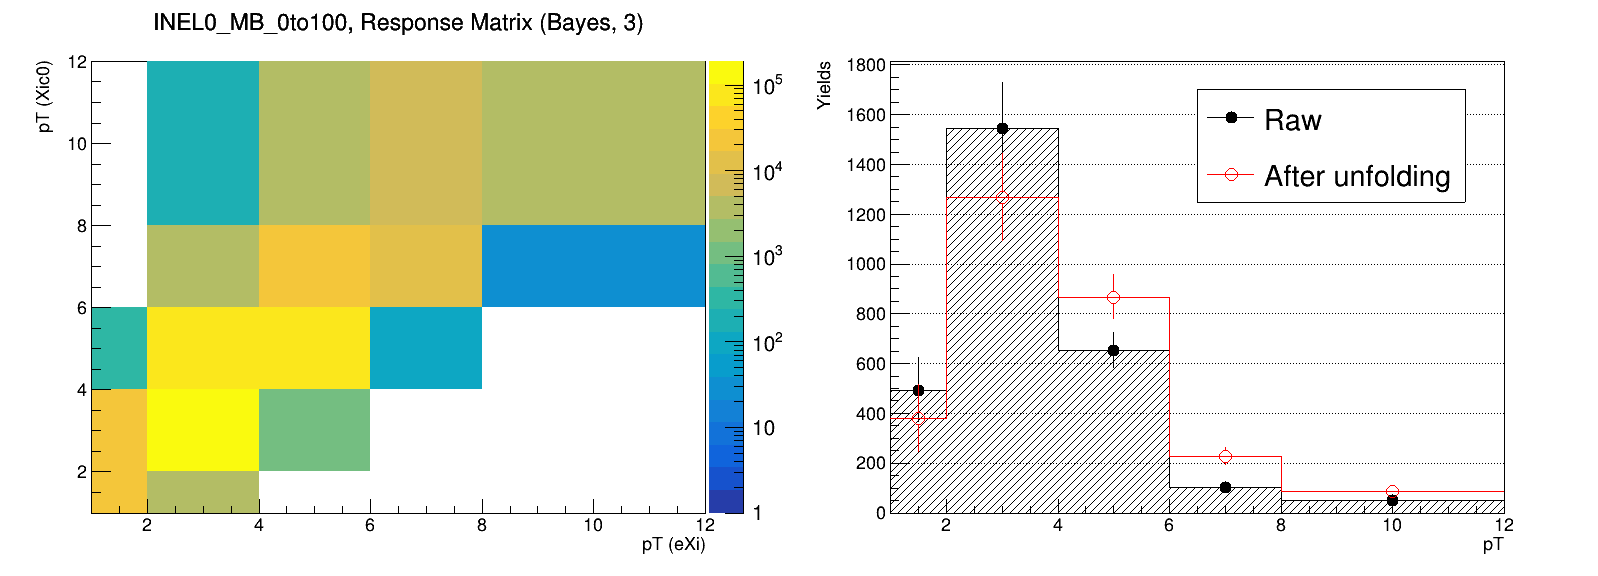
\includegraphics[width=0.95\textwidth]{plots/s2_unfold_INEL0_MB_0to100.png}
    \caption{\Xic - e\Xim response matrix by MC (left) and yields before and after the unfolding (right)}
    \label{fig:s2_unfolding}
\end{figure}

\clearpage
%++++++++++++++++++++++++++++++++++++++++++++

\vspace{\columnsep}
\paragraph{\blue{\Xic efficiency correction}}\mbox{}\\[1pt]
\red{TBU} \\

\begin{figure}[h]
    \centering
    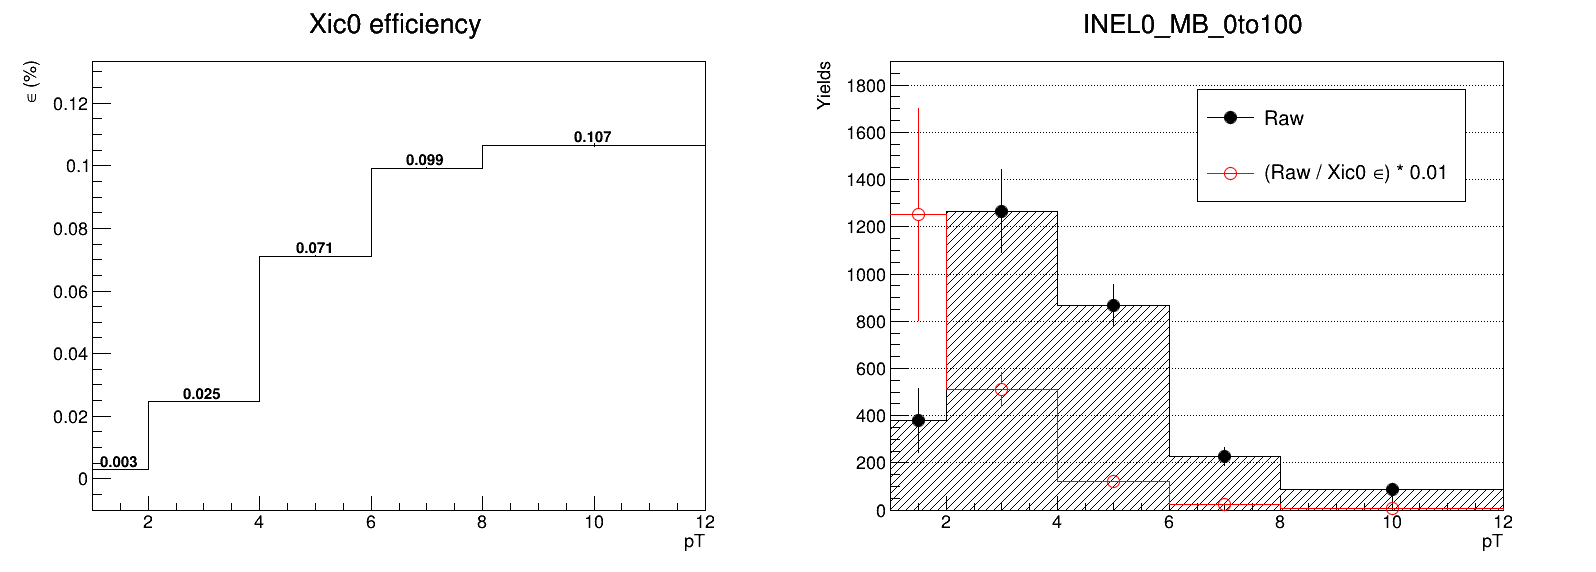
\includegraphics[width=0.95\textwidth]{plots/s2_Xic0Eff_INEL0_MB_0to100.png}
    \caption{$Acc \times \epsilon$ of \Xic (left) and Yields before and after correction (right)}
    \label{fig:s2_Xic0Eff}
\end{figure}

\clearpage
%++++++++++++++++++++++++++++++++++++++++++++

\paragraph{\blue{Feed-down subtraction}}\mbox{}\\[1pt]
\red{TBU}

\clearpage
%--------------------------------------------------------

\subsubsection{Crosscheck with previous analysis results} \label{subsubsec:xCheck}
%
As mentioned earlier in section \ref{sec:recap}, this analysis follows almost same analysis strategy by the previous \Xic $\rightarrow$ e\Xim analysis for \pp 13 \TeV. To ensure the validity of this study in addition to crosscheck the previous result, the overall analysis processes were cross-checked step by step, and then directly compared by using \Xic cross-section.
%
\begin{itemize}
    \small
    \item [] \blue{Crosscheck conditions} \vspace{1pt}
    \item[-] Target: MB inclusive (no multiplicity selection) \Xic cross-section
    \item[-] Online event selection: shared same Lego train output (section \ref{subsec:dataset}) \vspace{1pt}
    \item[-] Offline event selection: \\
     1. Uses each analyzer's codes \\
     2. Same cuts and factors (e.g., weighting factor for \pt spectra of MC) \vspace{1pt}
    \item[-] Offline analysis: \\
     1. Uses each analyzer's codes \\
     2. Same cuts and factors (e.g., Xic $\rightarrow$ e\Xim branching ratio) \\
     3. Same analysis steps (section \ref{subsubsec:onSel} - \ref{subsubsec:offAna}) are applied
\end{itemize}
%
The results of crosscheck are shown in Fig. \ref{fig:s2_xCheck}. The maximum deviation is smaller than 0.5 \%. Note that some factors applied are not necessarily the final one (e.g., Weighting factor for \pt spectra of MC) and among the analysis routines Feed-down subtraction was not applied.

\vspace{\columnsep}
\begin{figure}[h]
    \centering
    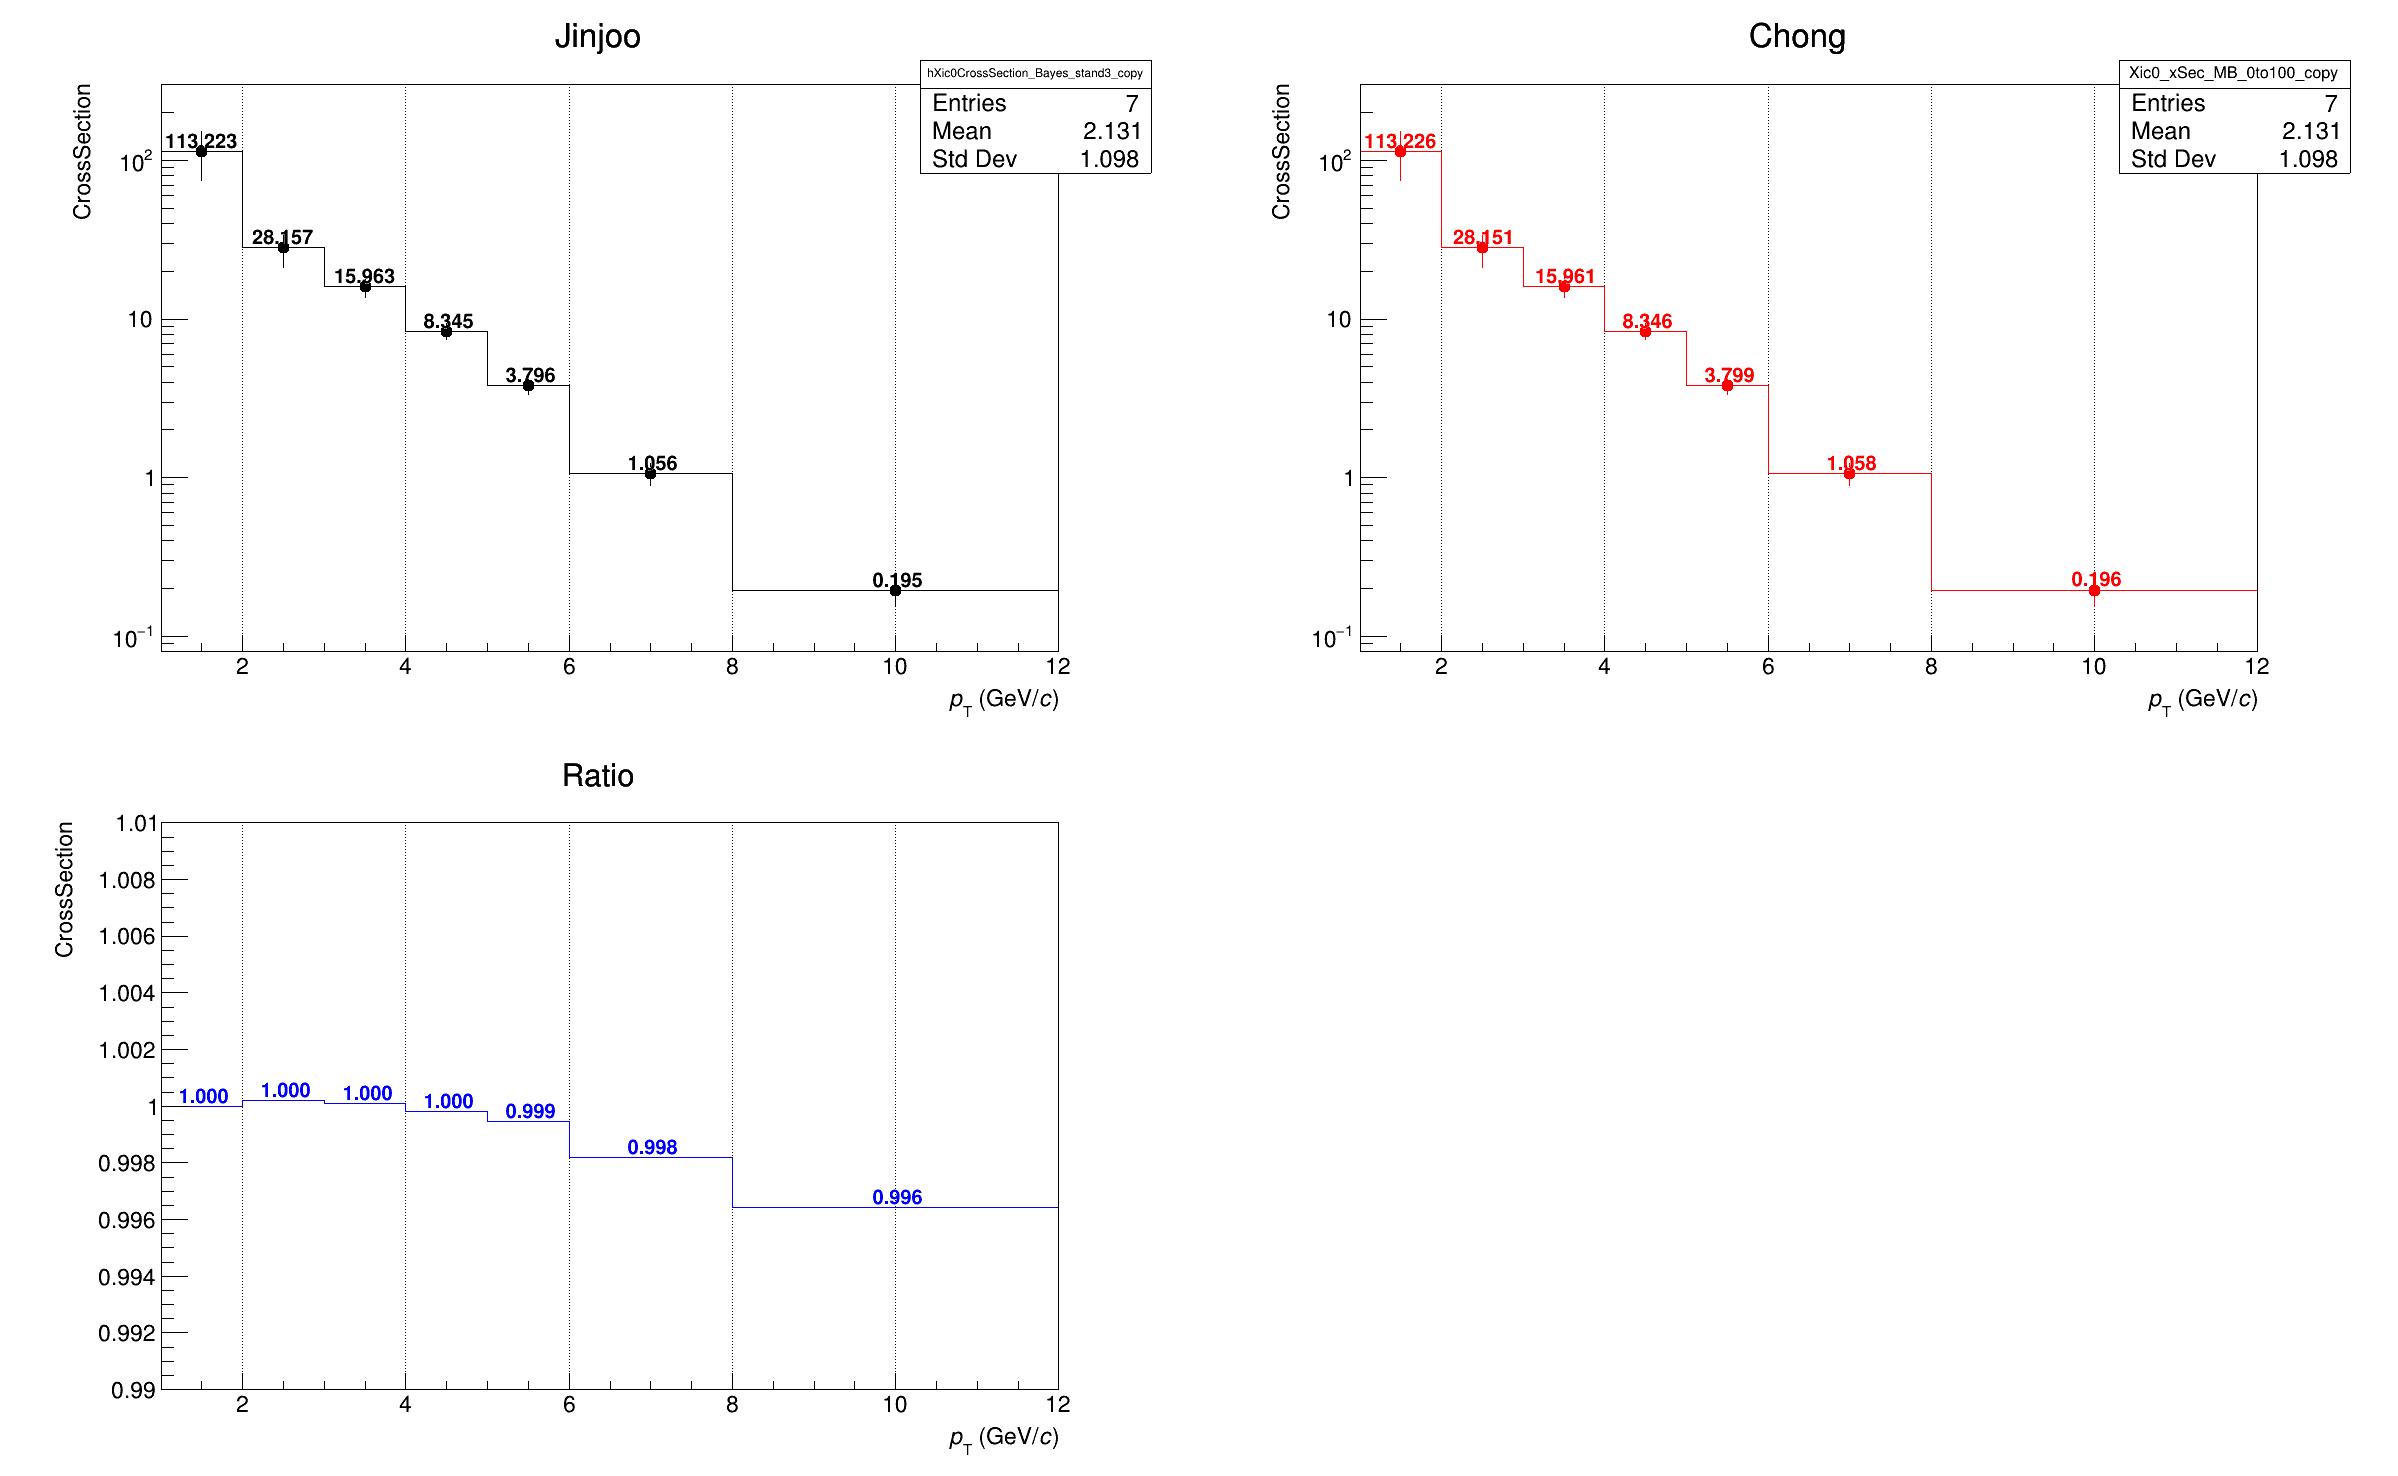
\includegraphics[width=0.95\textwidth]{plots/s2_xCheck.png}
    \caption{The crosscheck results: top left plot shows the \Xic cross-section by previous analysis, top right plot shows the same observable by this analysis, and bottom left shows the ratio between the them.}
    \label{fig:s2_xCheck}
\end{figure}